\documentclass[12pt]{article}

\usepackage{sbc-template}
\usepackage{graphicx,url}
\usepackage[utf8]{inputenc}
\usepackage[brazil]{babel}
\usepackage[latin1]{inputenc}  
\usepackage{float}
%\usepackage{natbib}
%\bibliographystyle{abbrvnat}
%\setcitestyle{authoryear,open={[},close={]}} 

     
\sloppy

\title{Ferramenta de Visualização de Dados\\ do Censo da Educação Superior do INEP}

%\author{Maria\inst{1}, Gui\inst{1}, Luciana\inst{2}, Isa\inst{1} }
\author{Guilherme Tomaselli Borchardt\inst{1}, Maria Teresa Silva Santos\inst{1},\\ Luciana Bolan Frigo\inst{2}, Isabela Gasparini\inst{1}}

\address{Departamento de Ciência da Computação – Universidade do Estado de Santa Catarina \\(UDESC) – Joinville – SC – Brasil 
 \nextinstitute{
 Departamento de Computação – Universidade Federal de Santa Catarina (UFSC) – \\Araranguá – SC – Brasil
 }
   \email{\{guilherme.borchardt,maria.santos2805\}@edu.udesc.br,}
   \email{luciana.frigo@ufsc.br, isabela.gasparini@udesc.br}
}

\begin{document} 

\maketitle

\begin{abstract}
  Educational data from Brazilian higher education are made available by INEP in CSV format, but their large volume makes the search for information onerous. In order to assist in this search and bring an understanding of the data, the tool that is still under development is presented. For its construction and foundation, a survey of related works on visualization tools was carried out. In the usability scenarios, the advantages and ease of visualization, interpretation and their contributions are observed. As future work, improvements are proposed in terms of usability and number of graphical information presented, in addition to evaluation with the user for effective improvement of the tool.
\end{abstract}
     
\begin{resumo} 
%max 10 linhas
    Os dados educacionais do ensino superior brasileiro são disponibilizados pelo INEP em formato CSV, porém seu grande volume torna a busca por informações onerosa. Visando auxiliar nessa busca e trazer um entendimento sobre os dados, apresenta-se a ferramenta que segue em desenvolvimento. Para sua construção e fundamentação realizou-se um levantamento de trabalhos relacionados sobre ferramentas de visualização. Nos cenários de uso, observam-se as vantagens e facilidades na visualização, interpretação e suas contribuições. Como trabalhos futuros propõe-se melhorias nos quesitos de usabilidade e número de informações gráficas apresentadas, além de avaliação com o usuário para efetivo aperfeiçoamento da ferramenta. 
   %Tendo em mente as dificuldades de visualização e interpretação de grandes dados, o presente artigo traz como proposta a implementação de uma ferramenta web para a visualização de dados educacionais do ensino superior apresentados pelo INEP.
\end{resumo}


\section{Introdução}\label{introdução}
Análises e visualizações acerca de dados educacionais, em uma esfera pública, possuem relevância social, levando em consideração aspectos de impacto tanto em políticas públicas, investimentos e comoção popular. A educação superior brasileira é uma grande geradora de dados, visualizá-los e correlacioná-los de forma clara e rápida que ilustram e destacam aspectos de relevância, especialmente para usuários que não fazem parte do campo da informática, para \cite{marx:2013}, continua sendo um desafio complexo. 

No Brasil, a entidade responsável por fornecer e iniciar pesquisas, estudos e avaliações sobre o sistema de educação é o Instituto Nacional de Estudos e Pesquisas Educacionais Anísio Teixeira (INEP). A partir de dados educacionais disponibilizados trazem análises sobre a Educação Superior.

Com a enorme quantidade de dados que são gerados diariamente, os dados abertos se tornaram cada vez mais comuns em nossas vidas, sendo assim um desafio democratizar as visualizações e realizar análises sobre tais informações. Segundo \cite{macedo:2020} a exploração dos dados abertos ainda é uma tarefa difícil para boa parte da população, muito em função do formato em que são publicados nos portais do governo, sendo geralmente disponibilizados em forma de tabelas contendo grandes volumes de dados.

O presente trabalho utiliza os dados da educação superior gerados pelo INEP, tendo em vista a dificuldade de interpretação e entendimento dos dados disponibilizados, apresenta-se então a proposta e implementação de uma ferramenta\footnote{https://github.com/guitomaselli07/Analisador\_Educacao\_Superior\_2019} de visualização, em formato \textit{web} e \textit{open source}, onde o usuário é livre para selecionar quais universidades deseja obter informações e recebe como retorno gráficos comparativos de idade, gênero, cor/raça e situação acadêmica de estudantes e professores. Vale  salientar que todas as classificações e palavras utilizadas para a criação dos filtros e gráficos vem diretamente do banco de dados, logo, as variáveis mostradas são feminino e masculino, bem como as variáveis de cor/raça e formas de ingresso.

Este artigo está estruturado como segue, para abordagem dos conceitos iniciais, a seção 2 apresenta os fundamentos da visualização de dados gerais, dados educacionais e as informações a serem extraídas do dado. Na seção 3 expõe alguns trabalhos que se relacionam com o tema proposto. Na seção 4 apresenta-se a ferramenta proposta em desenvolvimento, bem como as ferramentas tecnológicas auxiliares empregadas e os tratamentos sofridos pelos dados educacionais. A seção 5 discorre os resultados esperados para a pesquisa e os trabalhos futuros e por fim, na seção 6 são relatadas as considerações finais.

\section{Fundamentos}\label{fundamentos}
%falar um pouco dos datasets e embasar em como foi montado a ferramenta, pois ja sai falando das analises dos datasets.. trazer o mais inicial.
%pq usar cortado.
Os dados analisados provindos do INEP, utilizam-se também de outra base de dados, o Cadastro Nacional de Cursos e Instituições de Educação Superior, disponíveis no e-MEC\footnote{https://emec.mec.gov.br/}, que armazena os códigos dos cursos e das respectivas instituições.  Para tornar a ferramenta mais usual, fez-se um cruzamento de dados, onde o que fica visível na ferramenta  é o nome das instituições e o nome dos cursos, não apenas os códigos, o que dificultaria o processo de busca. Por sua vez, a ferramenta também disponibiliza a opção de campos editáveis, onde a busca funciona através destes códigos, o que é melhor apresentado na seção \ref{documetacaoDados}.

A ferramenta proposta realiza a apresentação de análises gráficas no contexto da educação superior, ressaltando a diferenciação entre os gêneros, tendo em vista a grande desigualdade entre a presença masculina e feminina, principalmente nos cursos de exatas. Segundo os dados do INEP de 2013, os cursos das áreas das exatas no Brasil são predominantemente mais procurados e frequentados por homens. Entre todos os cursos dessa área do conhecimento, é observado especialmente que o curso de Ciência da Computação chega a ter cerca 79,9\% de participação masculina, enquanto as mulheres representam uma parcela mínima no curso \cite{lima:2013}. %médio...

Para a construção dos gráficos atualmente presentes na ferramenta proposta, utilizou-se dos princípios do Design Universal, termo utilizado pela primeira vez na década de noventa pelo arquiteto americano Ronald Mace \cite{cud:2002}, possibilitando maior abrangência na identificação e visualização dos conteúdos apresentados. Para isso, todos os gráficos utilizaram-se das cores complementares, além da adição de diferentes texturas para a visualização das informações em preto e branco.

%FAZER UM FECHAMENTO DOS FUNDAMENTOS
%A visualização dos dados é uma parte muito importante para o desenvolvimento de um trabalho coeso e de fácil entendimento, pois é o que possibilita aos usuários transformar os dados em informações \cite{stasko:2008}.
% Nas análises sobre dados de um determinado \textit{dataset}, a utilização de gráficos em sua maioria são mais eficientes para a exploração e observação das informações. Um exemplo disso, é a utilização dos gráficos de barras, por possibilitarem que o usuário observe um contexto geral e possa sozinho fazer análises quantitativas sobre os dados apresentados. \cite{tufte:2001}.

Ter acesso a tais dados permite a avaliação real sobre a educação brasileira, diminuindo a distância do usuário com as universidades, mostrando um panorama geral de quem as frequenta e de seus professores. Amenizando também a dificuldade de interpretação sobre grandes planilhas, pois segunda \cite{macedo:2020} existe uma grande diversidade de formatos de visualização e as gráficas são fortemente recomendadas para esse tipo de situação.

\section{Trabalhos Relacionados}\label{trabalhosRelacionados}
Uma série de ferramentas para visualização de dados com cunho social são observadas na literatura, uma delas foi a proposta de ferramenta de visualização de dados abertos do portal de transparência da câmara dos vereadores de Florianópolis em \cite{santos:21}. As autoras propõem, a partir de dados expostos em formato de PDF, toda a conversão e processo para transformar tabelas descritivas em um \textit{dashboard} interativo com o retorno de gráficos e informações.

Em um contexto educacional, levando em conta o desafio da evasão escolar, formas computacionais de identificar possíveis estudantes que tendem a evadir, possibilitam às Instituições de Ensino Superior (IES) a reverter tal situação. Dessa forma, os autores \cite{barros:2017} apresentaram estudos sobre como ferramentas de visualização aliadas a técnicas estatísticas e de aprendizagem de máquina, podem influenciar na interpretação dos resultados obtidos. Para isso, os autores analisaram os dados educacionais pertencentes aos cursos de Licenciatura em Espanhol e Técnico de Segurança do Trabalho do Instituto Federal do Rio Grande do Norte, durante o período dos anos de 2008 até 2016.

Em uma situação de aplicabilidade distinta a proposta no presente artigo, \cite{zoppi:2021} apresenta uma ferramenta web (MiBiOmics) \textit{Open Access} de visualização de grandes dados relevantes para a área da biologia para uma análise integrativa e que gera novos \textit{insights} para seus usuários. Para \cite{zoppi:2021} o maior desafio na construção da ferramenta foi a diversidade técnica das formas de visualização e interpretação dos dados. Além disso, também aponta que muitas ferramentas de visualização não são acessíveis a seus usuários, neste caso os biólogos, que não possuem habilidades de programação de computadores. Como resultados, a equipe de pesquisadores apresenta a aplicação web que facilita a visualização, exploração, integração e análise de dados. 

Como panorama geral do tema, encontra-se na literatura o mapeamento sistemático sobre os dados abertos educacionais do Brasil, onde os autores \cite{ferreira:2021} analisaram as quantidades de bases de dados abertas utilizadas entre os anos de 2010 até 2021, e com isso puderam concluir diversos aspectos relevantes, como quais foram as bases mais requisitadas, até discussões sobre a necessidade de mais investimentos em ferramentas ou produtos voltados a entrega de melhores visualizações sobre os dados educacionais para gestores, professores e comunidade como um todo. Evidenciando assim a importância do desenvolvimento de mais soluções como a ferramenta proposta neste artigo.

\section{Ferramenta Proposta}\label{ferramentaProposta}
Utilizando os dados do INEP referentes ao Censo da Educação Superior de 2019, a ferramenta realiza a leitura, análise e apresentações gráficas sobre os dados, sempre priorizando as análises entre os gêneros. Além disso, a aplicação possibilita ao usuário, escolher diversos filtros para realizar as pesquisas, como escolher entre estudantes ou professores, especificar qual instituição de ensino, curso e também quais análises deseja gerar.

Como já foi citado anteriormente, um dos propósitos para o desenvolvimento da ferramenta é a democratização das informações sobre os dados da educação superior brasileira, levando em consideração que para realizar tal tarefa, boa parte da população pode apresentar certas dificuldades, principalmente em função dos códigos que são apresentados nas bases de dados, os quais são explicados no dicionário de variáveis disponibilizado pelo INEP, como o exemplo da variável TP\_SEXO que pode assumir apenas um valor, onde  \textit{1} representa os estudantes do sexo feminino, \textit{2} os estudantes do sexo masculino ou \textit{nulo}, onde o valor não foi informado.

\subsection{Documentação do Instituto Nacional de Estudos e Pesquisas Educacionais Anísio Teixeira (INEP)}\label{documetacaoDados}
No site do INEP é possível encontrar diversas bases de dados abertas ao público, sendo que uma delas é o Censo da Educação Superior que é divulgado todos os anos. Entre todos os Censos já divulgados, para a construção das análises presentes na ferramenta proposta, utiliza-se os dados do ano de 2019, com o intuito de analisar os dados mais recentes divulgados sobre a educação superior brasileira.

Dentre os arquivos presentes no documento dos microdados da educação superior de 2019, utilizam-se para realização das análises os seguintes arquivos do INEP: SUP\_ALUNO\_2019 e SUP\_DOCENTE\_2019. O primeiro arquivo é composto por 12.350.832 linhas e 112 colunas que são referentes aos dados dos estudantes. Já o segundo, aos dados dos professores e é composto por 399.428 linhas e 41 colunas. Por se tratar de grandes conjuntos de dados, fez-se uma limpeza nas bases, sendo inicialmente escolhidas apenas as variáveis apresentadas na Tabela  \ref{tab:my-table} para as construções gráficas da ferramenta.

%e as variáveis inicialmente escolhidas para as construções gráficas da ferramenta são apresentadas na Tabela \ref{tab:my-table}.

\begin{table}[H]
\centering
\caption{Variáveis utilizadas nas análises com a base de dados do INEP}
\label{tab:my-table}
\resizebox{\textwidth}{!}{%
\begin{tabular}{|l|l|}
\hline
CO\_IES       & Código único de identificação da IES                       \\ \hline
CO\_CURSO     & Código único de identificação do curso gerado pelo E-MEC   \\ \hline
TP\_COR\_RACA & Tipo da cor/raça do estudante                                  \\ \hline
TP\_SEXO      & Informa o sexo do estudante                                    \\ \hline
TP\_SITUACAO  & Tipo de situação de vínculo do estudante no curso              \\ \hline
NU\_IDADE     & Idade que o estudante completa no ano de referência do Censo   \\ \hline
TP\_SEXO      & Sexo do docente                                            \\ \hline
NU\_IDADE     & Idade que o docente completa no ano de referência do Censo \\ \hline
TP\_COR\_RACA & Tipo da cor/raça do docente                                \\ \hline
TP\_SITUACAO  & Tipo da situação do docente na IES                         \\ \hline
\end{tabular}%
}
\end{table}

%\subsection{Ferramentas Tecnológicas Auxiliares}\label{ferramentasTecnologicas}
Para o desenvolvimento da ferramenta, utilizou-se como ambiente de desenvolvimento o \textit{Visual Studio Code}\footnote{https://code.visualstudio.com/}, com o uso da linguagem de programação \textit{Python} 3\footnote{https://www.python.org/} além das seguintes três  bibliotecas que são disponibilizadas pela própria linguagem: A primeira biblioteca foi o Pandas\footnote{https://pandas.pydata.org/}, utilizada para realizar a leitura e as análises dos dados, a segunda foi o \textit{Matplotlib}\footnote{https://matplotlib.org/}, que fez a construção e as plotagens gráficas, e por fim, a Pillow \footnote{https://python-pillow.org/}, que foi utilizada para carregar as imagens presentes na página de ajuda. Além de todas as bibliotecas, utilizou-se o \textit{framework} \textit{Streamlit}\footnote{https://streamlit.io/}, que permitiu o desenvolvimento de toda a interface gráfica e o upload para um servidor online, assim disponibilizando a ferramenta para todos.


% \subsection{Desenvolvimento da Ferramenta}\label{desenvolvimentoFerramenta}
% Com o uso de todos os dados educacionais citados na seção \ref{documetacaoDados}, além de todas as ferramentas tecnológicas comentadas na seção \ref{ferramentasTecnologicas}, foi possível realizar todas as etapas do desenvolvimento, indo da leitura dos dados até a publicação da ferramenta proposta, chegando-se assim no produto final que pode ser visualizado na Figura \ref{fig:pagina_inicial}.


\begin{figure}[H]
\centering
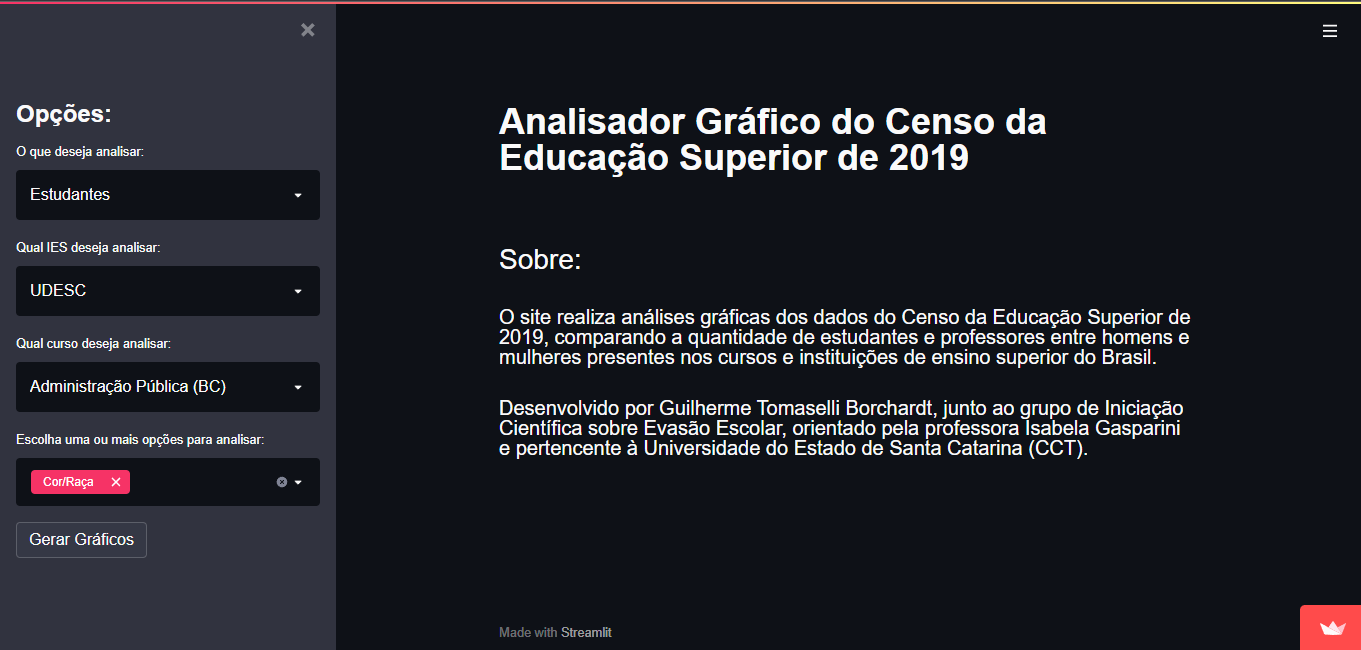
\includegraphics[width=1\textwidth]{pagina_inicial.png}
\caption{Página Inicial da Ferramenta Proposta}
\label{fig:pagina_inicial}
\end{figure}
%QUANDO FOR REFERENCIAR UMA FIGURA PODE USAR "Figura \ref{fig:pagina_inicial}". Desta forma podemos anexar outras figuras e o número de chamada sempre ficará correto.

A Figura \ref{fig:pagina_inicial} apresenta a página inicial da ferramenta. Inicialmente é apresentado no centro algumas informações relevantes, como por exemplo, de onde os dados foram retirados. Já na parte lateral esquerda da página, encontram-se os campos de pesquisas utilizados para a escolha de análise entre professores e estudantes, instituição de ensino, cursos e as análises que podem ser realizadas (gráficos de barras sobre cor/raça, idades e situações).

Caso o usuário escolha a opção "Outra", que está presente na caixa de seleção "Qual instituição deseja analisar", a ferramenta habilita o campo descritivo, onde o usuário pode inserir os dados referentes a determinada instituição de ensino e curso que deseja analisar, neste caso, a ferramenta apresenta o botão "Ajuda", o qual mostrará um passo a passo com imagens para auxiliar os usuários caso não saiba os códigos solicitados para executar a pesquisa.

A ferramenta proposta apresenta-se em fase de desenvolvimento, desta forma ainda não possui resultados referentes a seu uso por usuários. Apesar disso, os resultados esperados são positivos, visto facilitar o uso dos dados pela população.
 
\subsection{Resultados Gráficos da Ferramenta}

Após o usuário selecionar as opções de análise, presentes no canto esquerdo da tela, representado pela Figura \ref{fig:pagina_inicial}, a ferramenta apresentará os gráficos escolhidos pelo usuário. Sendo que os gráficos disponíveis são: número total de estudantes ou professor por cor/raça, idades e situações, sempre levando em conta a diferenciação entre os gêneros. 

Nesta fase de desenvolvimento, a ferramenta ainda está limitada à escolha e geração de três tipos de gráficos. Porém, a intenção para a continuação e evolução da ferramenta, é disponibilizar aos usuários uma maior quantidade de gráficos, com o intuito de possibilitar análises mais completas sobre os números entre estudantes ou professores na educação superior brasileira.

\begin{figure}[H]
\centering
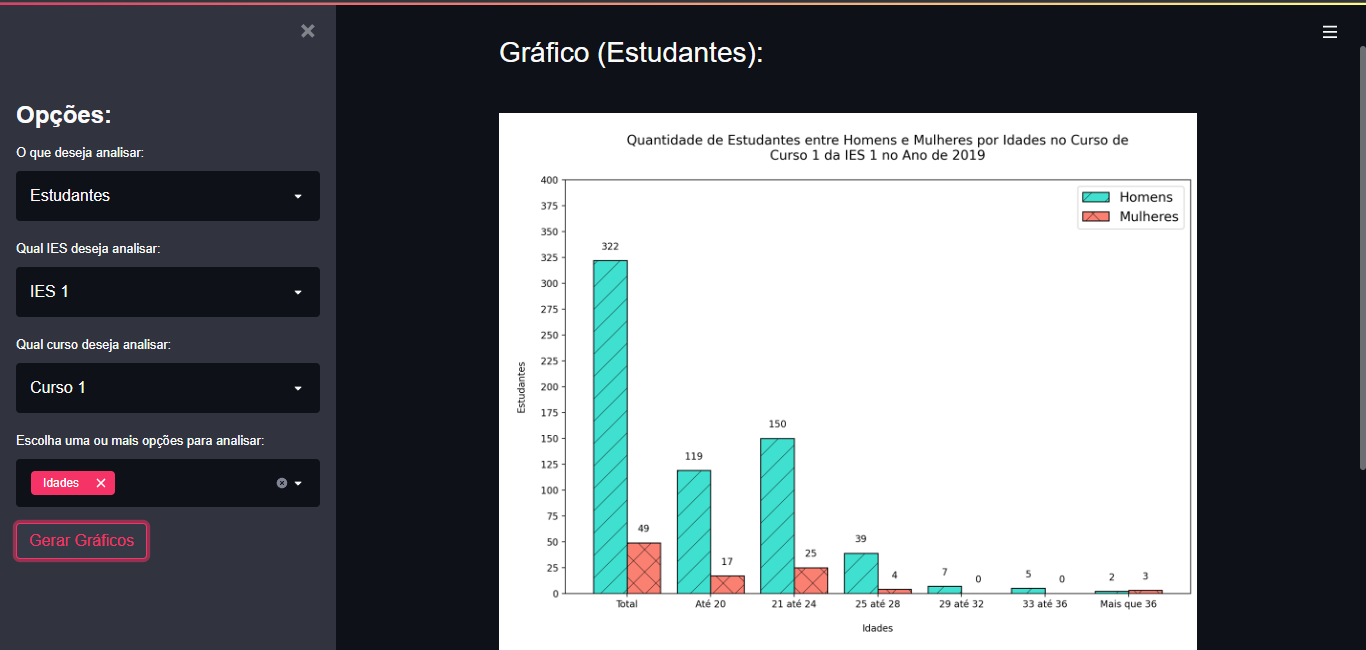
\includegraphics[width=1\textwidth]{grafico_com_interface.png}
\caption{Página Inicial da Ferramenta Proposta Após Clique no Botão Gerar Gráficos}
\label{fig:grafico_com_interface}
\end{figure}

%falar do gráfico AQUI

\begin{figure}[H]
\centering
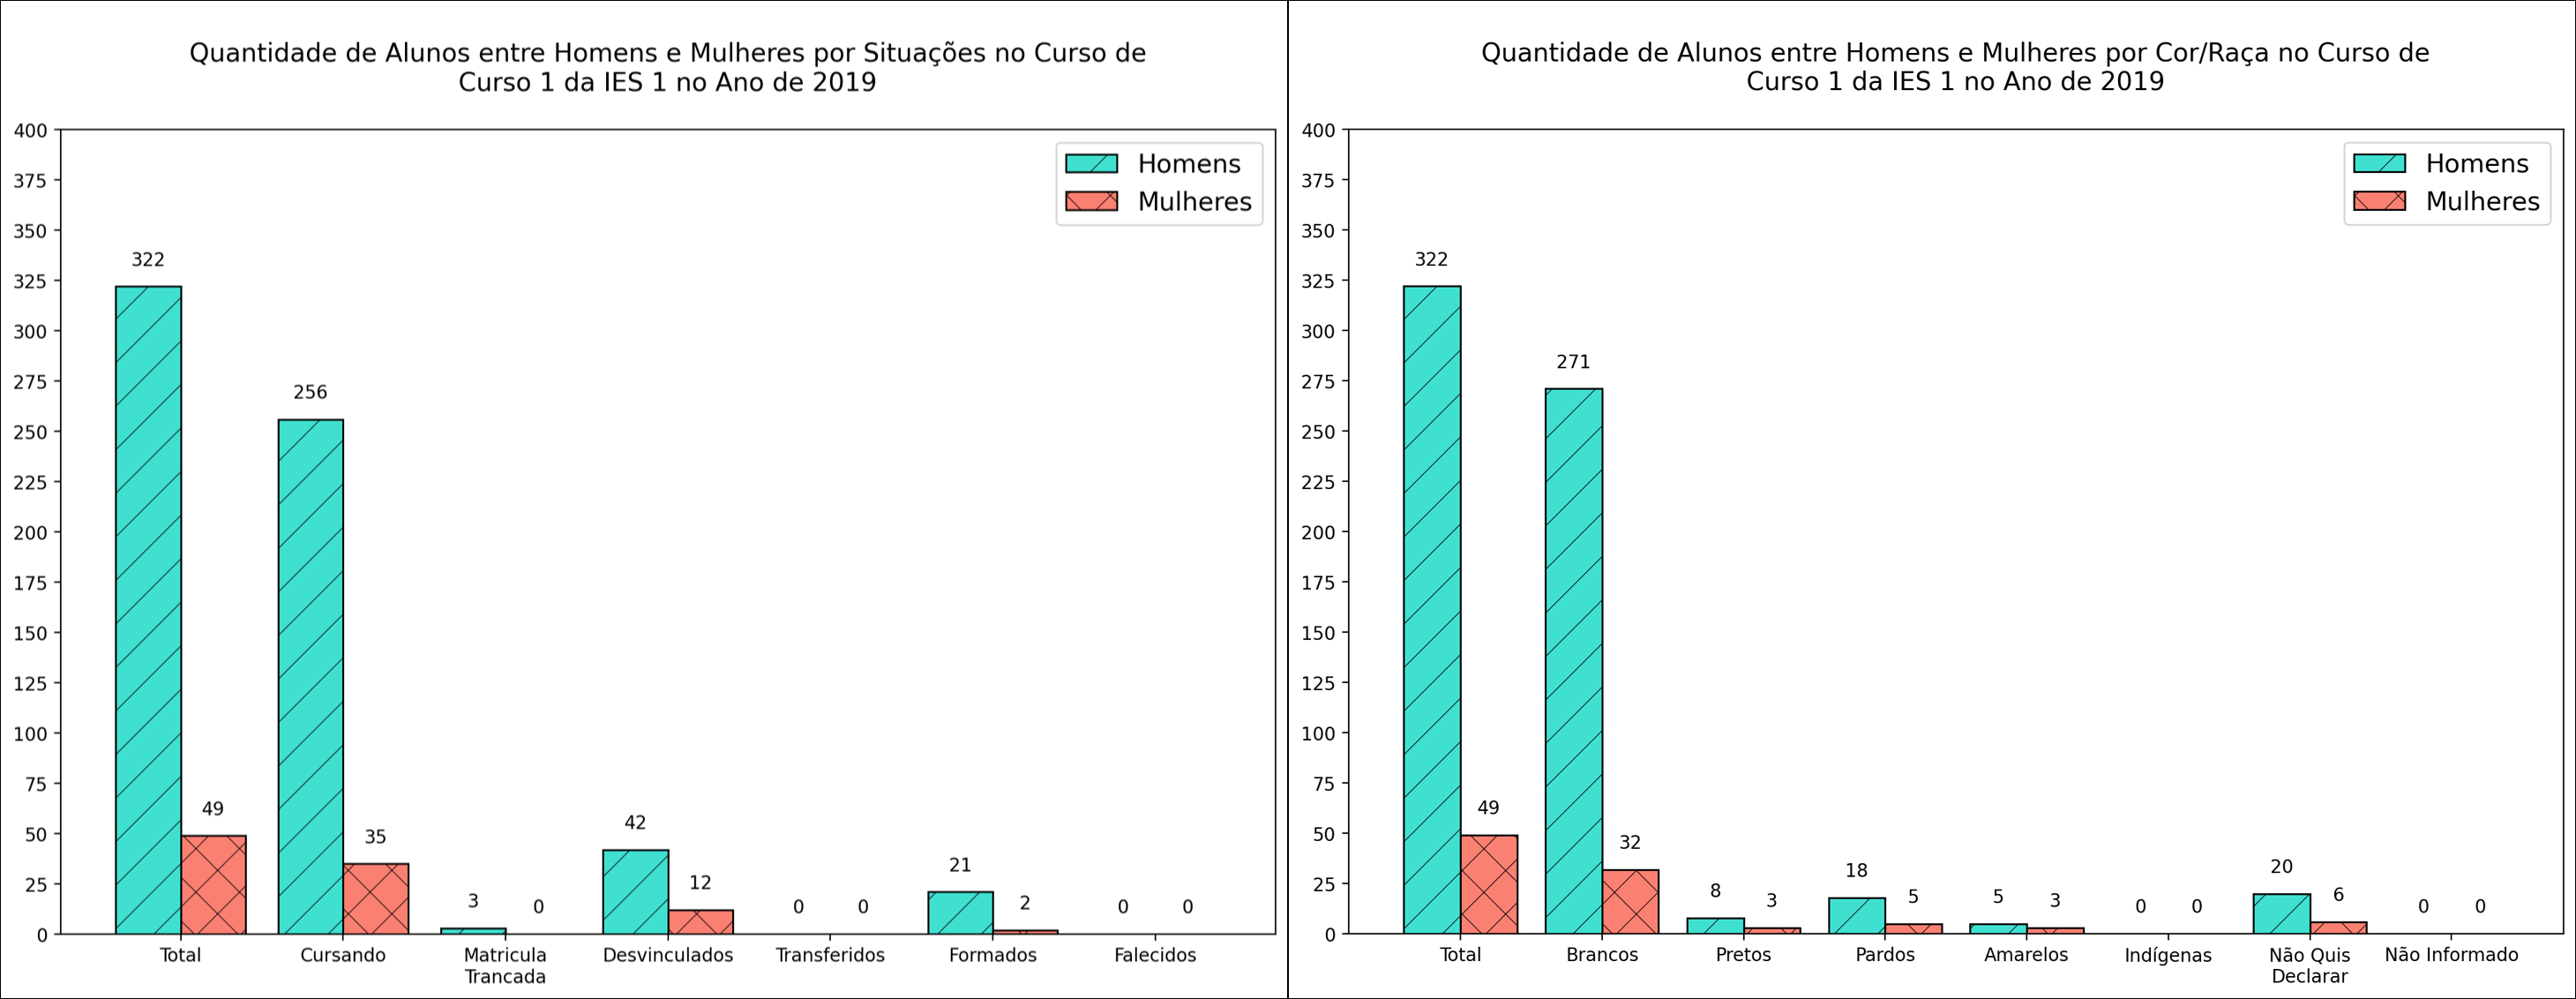
\includegraphics[width=1\textwidth]{grafico_raca_situacao.png}
\caption{Quantidade de Estudantes entre Homens e Mulheres por Situações de Curso e por Cor/Raça}
\label{fig:grafico_raca_situacao}
\end{figure}

As Figuras \ref{fig:grafico_com_interface} e \ref{fig:grafico_raca_situacao}, são exemplos de gráficos gerados pela ferramenta. Na Figura \ref{fig:grafico_com_interface} é possível observar a ferramenta em uso, onde o usuário inseriu as opções de análise, assim retornando como resultado o gráfico sobre as faixas etárias dos estudantes de uma determinada instituição de ensino e curso. Já a Figura \ref{fig:grafico_raca_situacao} mostra as outras duas possibilidades gráficas, que são sobre o número de estudantes por situações e cor/raça.
%falar do gráfico AQUI

%\begin{figure}[H]
%\centering
%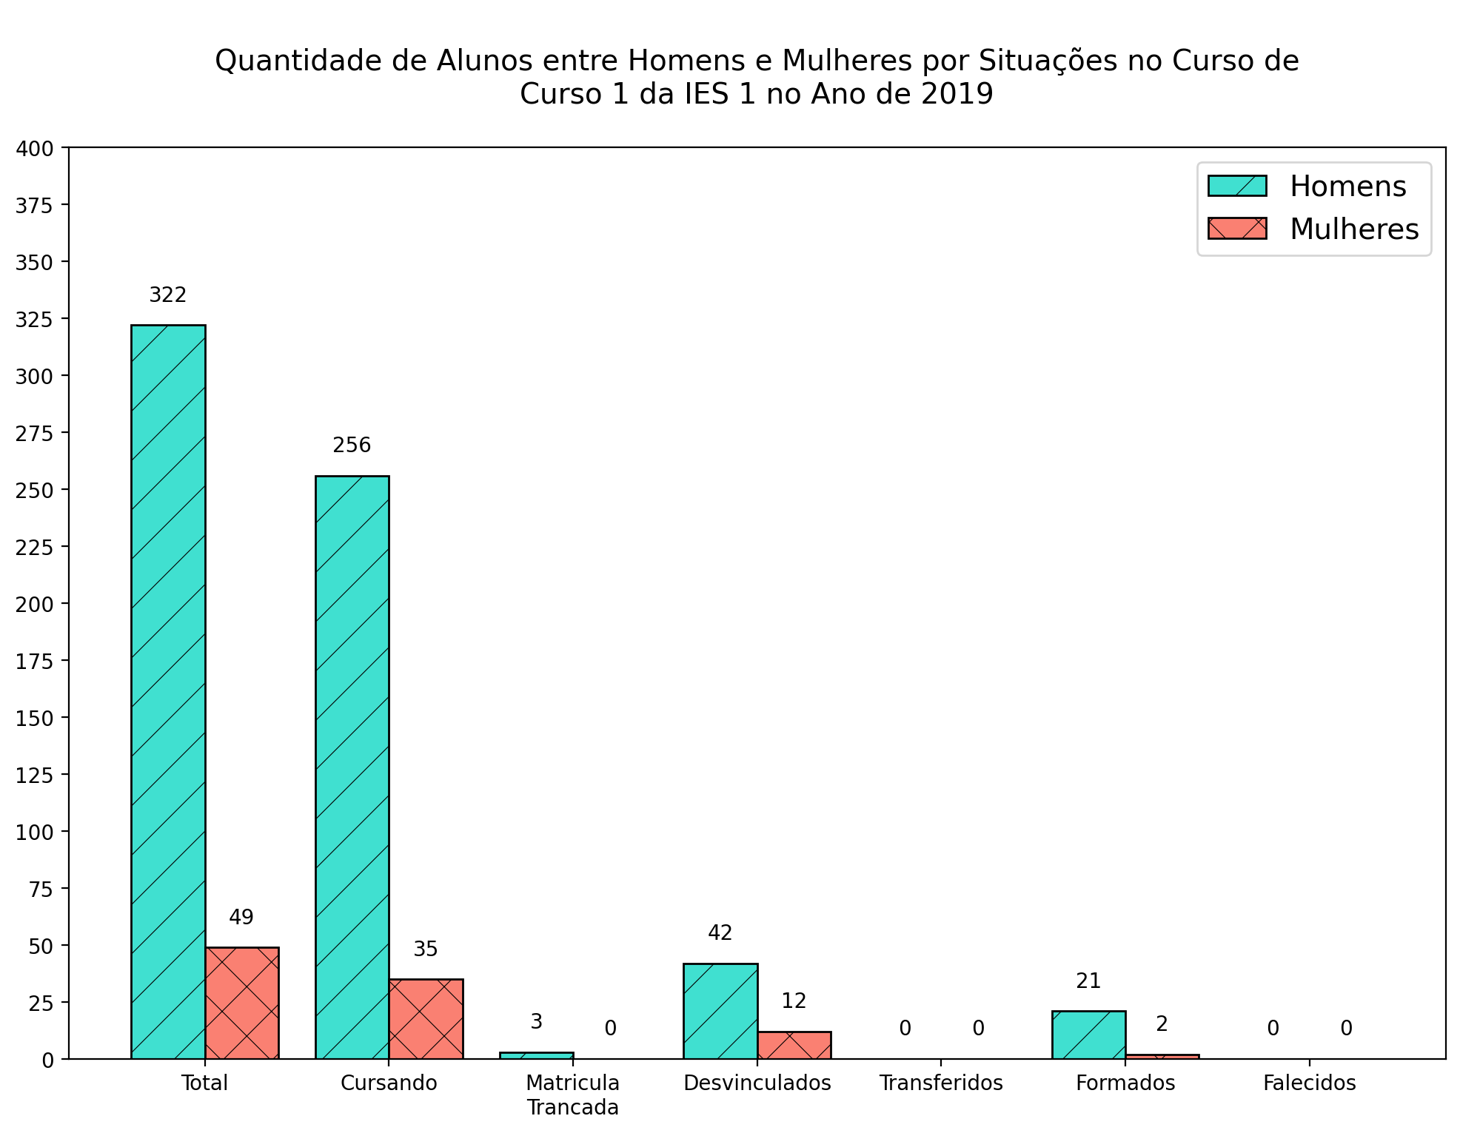
\includegraphics[width=.8\textwidth]{grafico_situacoes.png}
%\caption{Quantidade de Estudantes entre Homens e Mulheres por Situações de Curso no Curso de Curso 1 da IES 1 no ano de 2019}
%\label{fig:grafico_situacoes}
%\end{figure}

%falar do gráfico AQUI

%Os gráficos apresentados são x, y e z... Que representam m,n e p...

\section{Considerações Finais e Trabalhos Futuros}
%Como trabalhos futuros: interatividade gráfica, adicionar mais análises, gerar relatório pdf para impressão e compartilhamento, melhorar a ferramenta em si, etapas de teste com usuários e questionários, incluir análises de evasão escolar, incluir todos os anos dos dados INEP. 

Apresentou-se uma discussão sobre as dificuldades de interpretação de dados em forma de tabelas contendo um grande volume de dados. Apresentou-se também alguns trabalhos da literatura correlacionados com o tema proposto e por fim a apresentação da ferramenta proposta neste trabalho. Como contribuição, a ferramenta tem como principal intenção democratizar a análise de dados por usuário sem experiência no assunto, com apenas algumas seleções e cliques, recebe uma série de análises gráficas das instituições de ensino superior e cursos desejados.

Pretende-se com a ferramenta a constante atualização nas apresentações gráficas, sua construção conta com diversas propostas futuras, como a programação de gráficos interativos, a adição de diferentes análises, a opção de gerar um relatório para a impressão e compartilhamento dos gráficos em formato PDF, inclusão de todos os anos disponibilizados pelo INEP, possibilitando assim análises mais complexas, como por exemplo, análises mais detalhadas sobre evasão escolar. 
%Além das melhorias na ferramenta, propõe-se também a validação junto aos usuários, com a aplicação de questionário para o público interessado.  

%Como já mencionado anteriormente, utiliza-se dos dados do INEP referentes ao ano de 2019, com isso, toma-se como trabalhos futuros a apresentação das análises a partir do ano de 1995. Também almeja-se a aplicação de outros filtros para análises mais específicas do dado, bem como a melhoria do tratamento de erros provindos de sua utilização. 

Após a conclusão de trabalhos futuros relacionados com a etapa de desenvolvimento e melhorias da ferramenta, propõe a aplicação de avaliação com os usuários para verificação de dificuldades e facilidades do uso da nova forma de apresentação dos dados, fazendo comparações com a forma de visualização em tabelas e documentos, provindas dos dados do INEP e gráficos, provindos da ferramenta proposta.

\section{Agradecimentos}
Agradecemos o apoio do Conselho Nacional de Desenvolvimento Científico e Tecnológico (CNPq) 308395/2020-4,  Fundação de Amparo à Pesquisa e Inovação do Estado de Santa Catarina (FAPESC) Nº 027/2020 Apoio a Infraestrutura para Grupos de Pesquisa da UDESC TO n° 2021TR795 e Coordenação de Aperfeiçoamento de Pessoal de Nível Superior - Brasil (CAPES) - Código de Financiamento 001.


%\begin{figure}[ht]
%\centering
%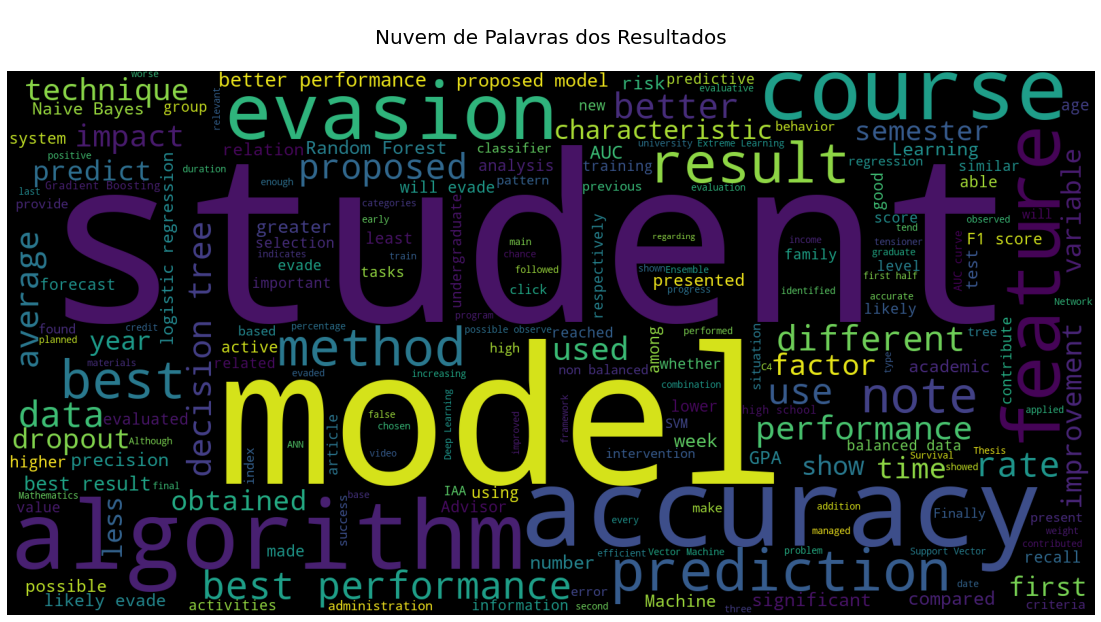
\includegraphics[width=1\textwidth]{fig2.png}
%\caption{This figure is an example of a figure caption taking more than one
 % line and justified considering margins mentioned in Section~\ref{sec:figs}.}
%\label{fig:exampleFig2}
%\end{figure}


\bibliographystyle{sbc}
\bibliography{sbc-template}


\end{document}




